\chapter{評価}
\label{evaluation}

本章では,提案システムの評価について述べる.


\section{評価内容}

本研究の実験において以下の項目について評価を行う.


\begin{itemize}
    \item DQNモデルによって出力された経路選択はユースケースに挙げた項目を満たせているか.
    \item ユースケース満たした上で, なるべく距離が短いルートを選択できているか.
\end{itemize}


\section{評価方法}

本研究では既存の距離

まず, DQNが選択した経路を表す出力~\ref{out:vector}を得る. 出力されたデータは入力と同じ17x17の正方行列である.
ここでは, 出力された行列を行動行列と定義し, この行動行列のうち0でない要素に行動が記録されているので, 図~\ref{out:vector}の矢印が記録された
要素を図~\ref{out:map}のように地図上の線分データに変換を行う.

\begin{figure}[htbp]
    \begin{minipage}{0.5\hsize}
        \begin{center}
            \includegraphics[width=70mm]{assets/action_vector.eps}
        \end{center}
        \caption{DQNが選択した経路を表す行列}
        \label{out:vector}
    \end{minipage}
    \begin{minipage}{0.5\hsize}
        \begin{center}
            \includegraphics[width=70mm]{assets/action_vector_visualize.eps}
        \end{center}
        \caption{交差点をマーク}
        \label{out:map}
    \end{minipage}
\end{figure}



%%% Local Variables:
%%% mode: japanese-latex
%%% TeX-master: "./thesis"
%%% End:
